\documentclass{article}

\usepackage[utf8]{inputenc}

\usepackage{nicefrac}
\usepackage{amssymb, amsmath, amsfonts}
\usepackage{amsthm}
\usepackage{tikz}
\usetikzlibrary{matrix,shapes,arrows, calc, intersections}
\usetikzlibrary{decorations.markings}
\usepackage{pgfplots}
\usepgfplotslibrary{groupplots}
\usepackage[a4paper, margin=1in]{geometry}

\newtheorem{proposition}{Proposition}
\newtheorem{theorem}{Theorem}
\newtheorem{definition}{Definition}
\newtheorem{lemma}{Lemma}
\newtheorem{conjecture}{Conjecture}
\newtheorem{corollary}{Corollary}
\newtheorem{remark}{Remark}
\newtheorem{assumption}{Assumption}

\newlength\figureheight
\newlength\figurewidth
\setlength\figureheight{12cm}
\setlength\figurewidth{14cm}

\newcommand{\tikzdir}[1]{tikz/#1.tikz}
\newcommand{\inputtikz}[1]{\input{\tikzdir{#1}}}

\DeclareMathOperator*{\argmin}{arg\; min}     % argmin
\DeclareMathOperator*{\argmax}{arg\; max}     % argmax
\DeclareMathOperator*{\tr}{tr}     % trace
\DeclareMathOperator{\Cov}{Cov}
\DeclareMathOperator{\logdet}{log\;det}

\title{EE8087 Living with Mathematics\\Tutorial 4: Conic Sections}
\date{}
\begin{document} \maketitle
\begin{enumerate}
\item For a conic curve described by the following quadratic equation:
  \begin{align*}
    x^2 + 6xy+9y^2 + 2x - 5y + 10=0. 
  \end{align*}
  Calculate the eccentricity of the curve.

\item For a paper strip $AB$ of length $20$. Suppose $A$ is on the $y$-axis and $B$ is on the $x$-axis. If $P = (6,6)$ is on the paper strip, find the coordinate of $A$ and $B$.
\begin{figure}[ht]
  \centering
  \begin{tikzpicture}[scale=0.3]
 \draw[->] (0,0) -- (10,0) node[right] {$x$};
  \draw[->] (0,0) -- (0,20) node[above] {$y$};

  \node [inner sep=0, outer sep=0, label=90:$P$] (P) at (6,6) {}; 
  \fill [black] (P) circle (4pt); 

  \node [inner sep=0, outer sep=0, label=180:$A$] (a) at (0,17.84) {}; 
  \fill [black] (a) circle (4pt); 
  \node [inner sep=0, outer sep=0, label=270:$B$] (b) at (9.04,0) {}; 
  \fill [black] (b) circle (4pt); 

  \draw [semithick] (a)--(b);
  \end{tikzpicture}
\end{figure}

\item We have 3 base stations at $A = (-5,0)$, $B = (0,0)$ and $C = (5,0)$. Suppose the signal sends by the each station travels at a speed of $1$ and the three base stations broadcast the signal simultaneously at an unknown time. The signals from stations $A$, $B$ and $C$ are received by a boat at time $3$, $0$, $4$ respectively. Find the position of the boat $P$.

  \begin{figure}[ht]
    \centering
    \begin{tikzpicture}
      \draw[->] (6,0) -- (-6,0) node[right] {$x$};
      \draw[->] (0,-1) -- (0,4) node[above] {$y$};

      \node [inner sep=0, outer sep=0, label=45:$P$] (P) at (-0.529,1.706) {}; 
      \fill [black] (P) circle (2pt); 
      \node [inner sep=0, outer sep=0, label=180:$A$] (a) at (-5,0) {}; 
      \fill [black] (a) circle (2pt); 

      \node [inner sep=0, outer sep=0, label=45:$B$] (b) at (0,0) {}; 
      \fill [black] (b) circle (2pt); 

      \node [inner sep=0, outer sep=0, label=270:$C$] (c) at (5,0) {}; 
      \fill [black] (c) circle (2pt); 

      \draw (a)--(P)--(c);
      \draw (b)--(P);
    \end{tikzpicture}
  \end{figure}
\newpage
\item We are building a Cassegrain reflector. Suppose the vertex of parabolic mirror is at $(0,0)$ and the vertex of the hyperbolic mirror is at $(5,0)$. The light is gathered at point $(-2,0)$. Find the equation describing the parabolic and hyperbolic mirrors.
  \begin{figure}[ht]
    \centering
    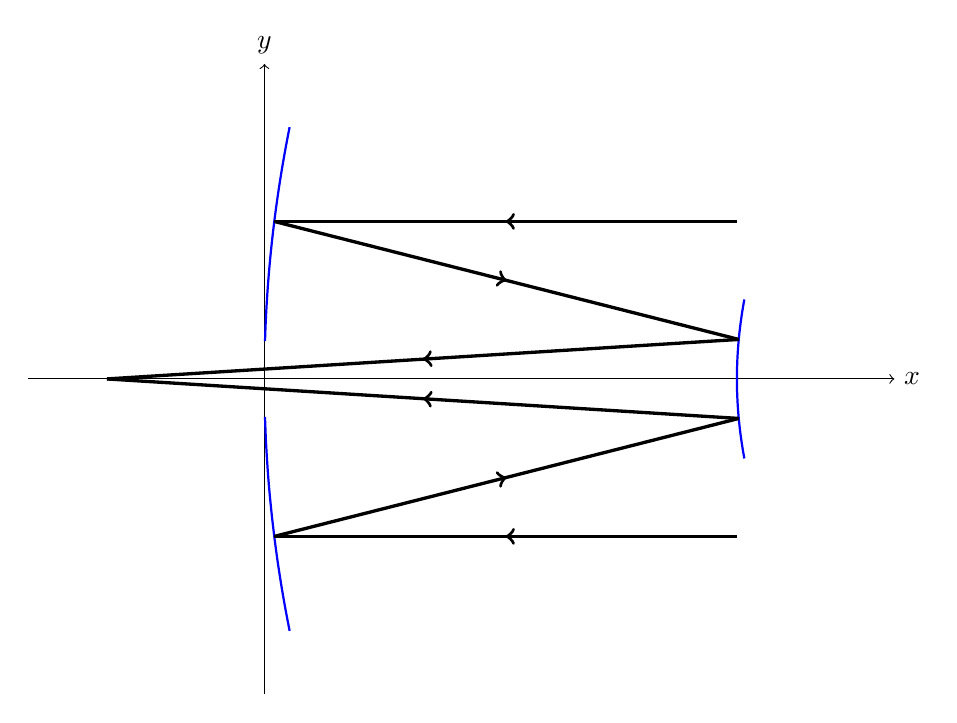
\begin{tikzpicture}
      \draw[->] (-3,0) -- (8,0) node[right] {$x$};
      \draw[->] (0,-4) -- (0,4) node[above] {$y$};

      \draw[name path=hyperbola, domain=-0.25:0.25, samples=20,smooth,variable=\t,blue,thick] plot ({3*cosh(\t)+3},{4*sinh(\t)});
      \draw[domain=-0.1:-0.015, samples=20,smooth,variable=\t,blue,thick] plot ({32*\t*\t},{32*\t});
      \draw[domain=0.015:0.1, samples=20,smooth,variable=\t,blue,thick] plot ({32*\t*\t},{32*\t});

      \path[name path=line1] (0.125,2)--(8,0);
      \path[name path=line2] (0.125,-2)--(8,0);
      \path[name intersections={of=line1 and hyperbola}];
      \begin{scope}[very thick,decoration={
          markings,
          mark=at position 0.5 with {\arrow{>}}}
        ] 
        \draw[postaction={decorate}] (6,2)--(0.125,2);
        \draw[postaction={decorate}] (0.125,2)--(intersection-1);
        \draw[postaction={decorate}] (intersection-1)--(-2,0);
      \end{scope}

      \path[name intersections={of=line2 and hyperbola}];
      \begin{scope}[very thick,decoration={
          markings,
          mark=at position 0.5 with {\arrow{>}}}
        ] 
        \draw[postaction={decorate}] (6,-2)--(0.125,-2);
        \draw[postaction={decorate}] (0.125,-2)--(intersection-1);
        \draw[postaction={decorate}] (intersection-1)--(-2,0);
      \end{scope}


    \end{tikzpicture}
  \end{figure}

\end{enumerate}

\end{document}
%%% Local Variables:
%%% TeX-command-default: "Latexmk"
%%% End:
